\NeedsTeXFormat{LaTeX2e}
\documentclass[10pt]{scrartcl}

\usepackage{tabularx,graphicx,listings,wrapfig,color,rotating}

\usepackage[vcentering,pdftex]{geometry}
\usepackage[absolute]{textpos}

\geometry{papersize={1220pt,860pt}}

\newcommand{\boxwidth}{5in}
\newcommand{\spacewidth}{604pt}
\setlength{\evensidemargin}{39.76274pt}
\setlength{\oddsidemargin}{39.76274pt}

\pdfcompresslevel=9
\def\pdfBorderAttrs{/Border [0 0 0] } % No border around Links
\usepackage{hyperref}

\begin{document}
\thispagestyle{empty}

\begin{textblock}{}(15.92,4.45)
  \begin{rotate}{270}
    \colorbox{red}{\textsf{\bfseries\Large\textcolor{white}{
          \hspace{2.09cm}Equalizer 0.6 Programming Guide\hspace{2.09cm}}}}
  \end{rotate}
\end{textblock}

\vfill
\parbox[t]{\spacewidth}{\hfill}
\parbox[t]{\boxwidth}{
  \center
  \textsf{\textbf{\huge Equalizer Programming Guide}}\\[\bigskipamount]
  {\Large Eyescale Software GmbH}
}\\
\vfill
\hspace{-128pt}
  \includegraphics[width=604pt]{images/teaserBack.pdf}
  \hspace{11pt}
  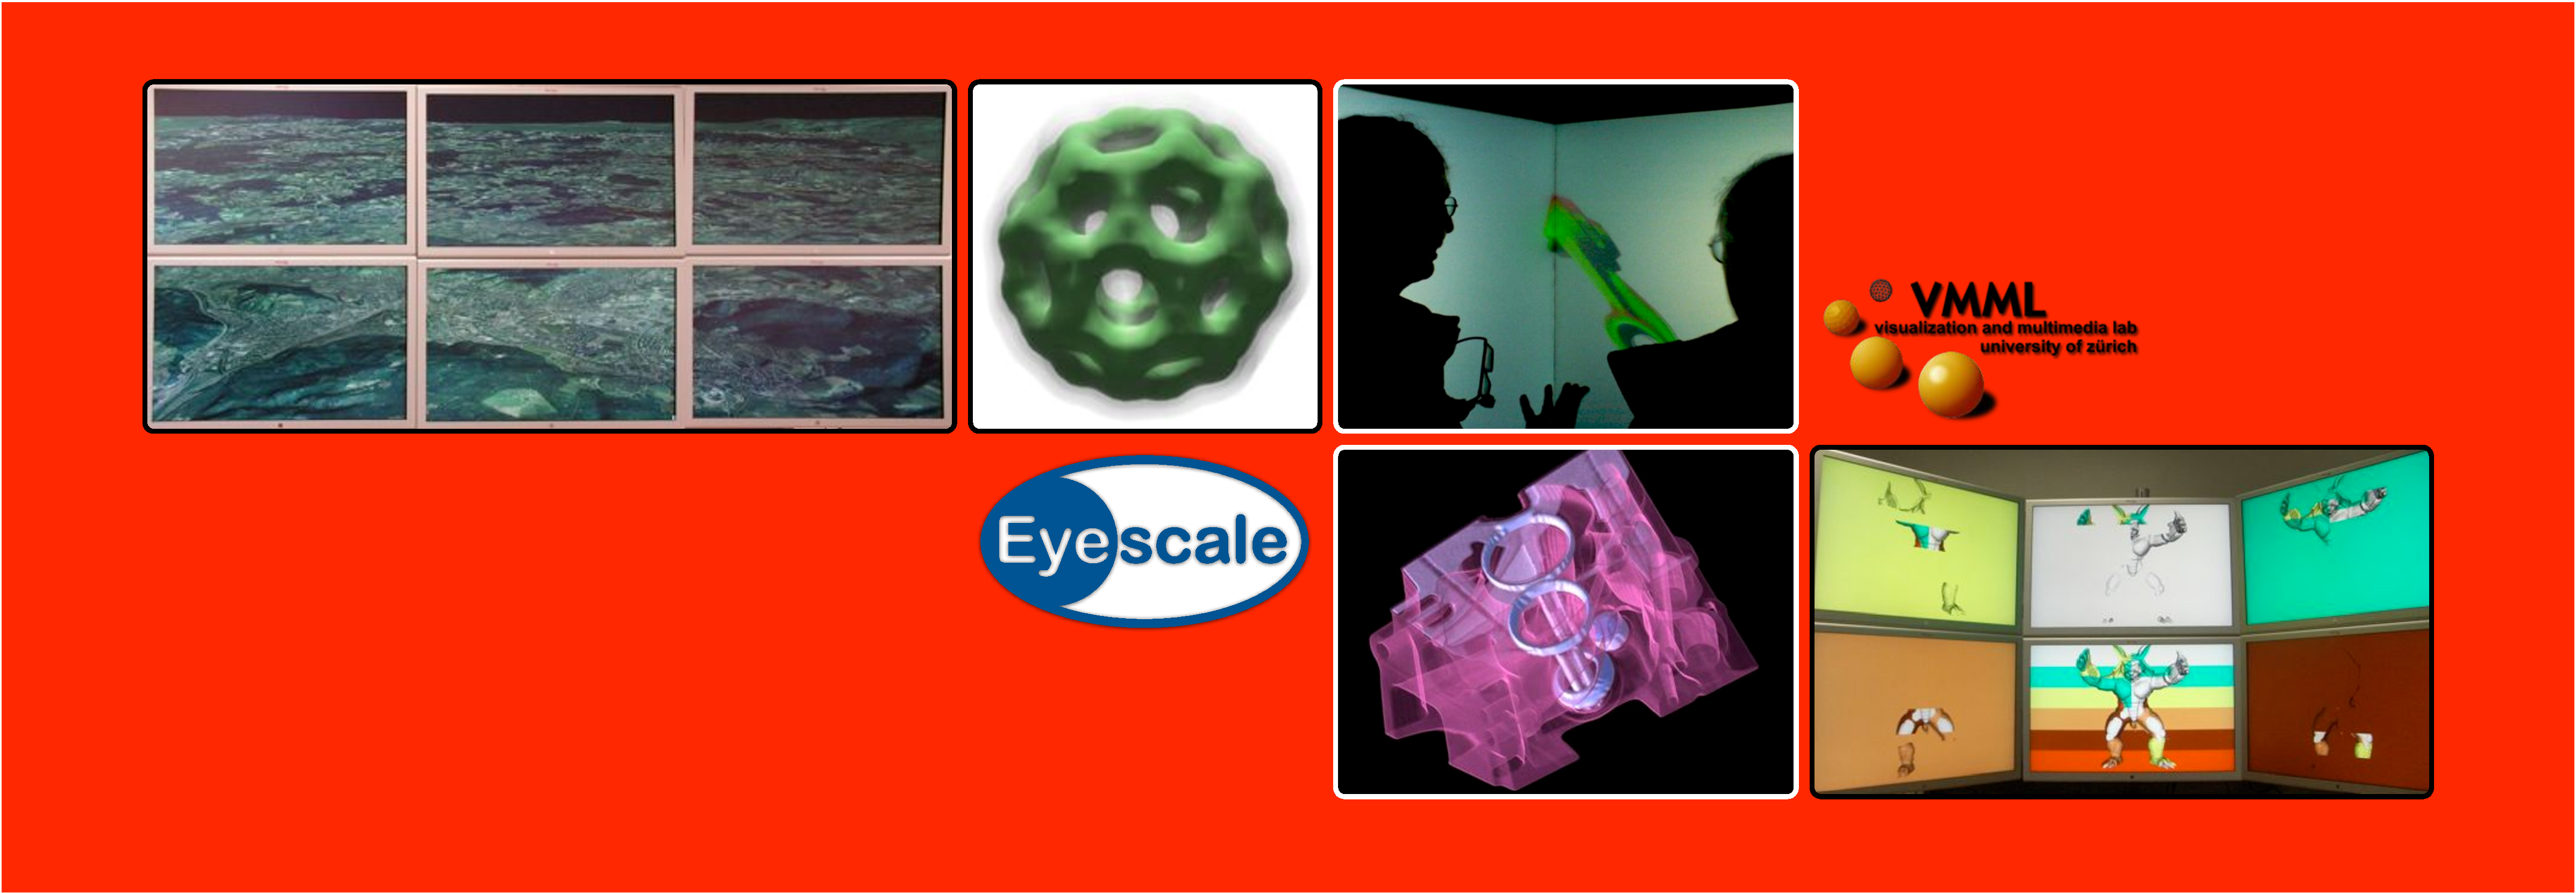
\includegraphics[width=604pt]{images/teaser.pdf}
\\
\vfill
\parbox[t]{\spacewidth}{\hfill}
\parbox[t]{\boxwidth}{ 
  {\Large\sffamily The official reference for creating parallel,
    scalable {OpenGL\texttrademark} applications with the Equalizer
    parallel rendering framework}\\\vspace{1cm}
  \center 
  {\Large Revision 1.4 for Equalizer 0.6}\\[\medskipamount]
}

\end{document}
